\section{实验}
假设噪声为高斯白噪声,并已知其均值 $0$,标准差为 $\sigma$。以下给出初始图像及噪声图像:
\begin{figure}[H]
\centering
\subfigure[原始图像]{\label{figure:001} 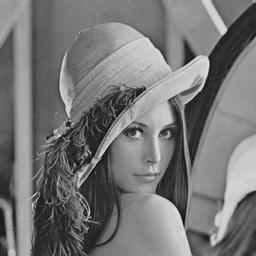
\includegraphics[width=0.4\textwidth]{001}}
\subfigure[噪声图像($\mu=0,\sigma=20$)]{\label{figure:002} 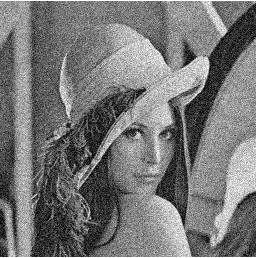
\includegraphics[width=0.4\textwidth]{002}}
\caption{初始图像及噪声图像}
\end{figure}

\subsection{实验1}
分别取 $\lambda=\frac{1}{20^2},\frac{10}{20^2},\frac{5}{20^2},\frac{20}{20^2},\epsilon=0.00001$,迭代 $50$ 次,得到结果如下:
\begin{figure}[H]
\centering
\subfigure[$\lambda=\frac{1}{20^2}$]{\label{figure:1/20} 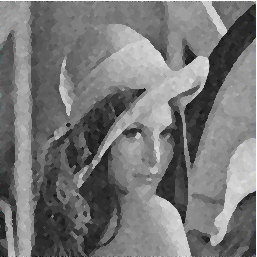
\includegraphics[width=0.4\textwidth]{003}}
\subfigure[$\lambda=\frac{5}{20^2}$]{\label{figure:5/20} 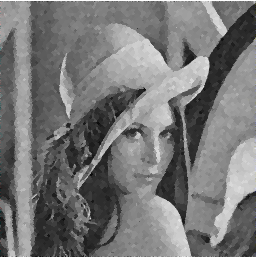
\includegraphics[width=0.4\textwidth]{004}}
\caption{第一组实验图}
\end{figure}
\begin{figure}[H]
\centering
\subfigure[$\lambda=\frac{10}{20^2}$]{\label{figure:10/20} 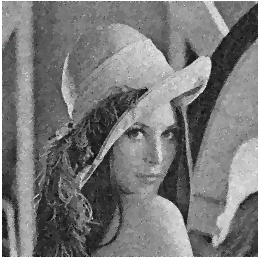
\includegraphics[width=0.4\textwidth]{005}}
\subfigure[$\lambda=\frac{20}{20^2}$]{\label{figure:20/20} 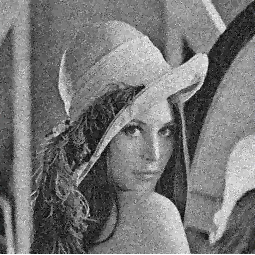
\includegraphics[width=0.4\textwidth]{006}}
\caption{第二组实验图}
\end{figure}
由上结果可以知道因为参数 $\lambda$ 对平衡去噪与平滑起到重要作用,因此参数 $\lambda$ 对于复原效果很重要。$\lambda$太小时,图像过度平滑以致边缘严重模糊;相反,$\lambda$ 太大时,图像去噪效果不好。
\subsection{实验2}
下面将本文算法与TV复原算法作比较,取 $\lambda=\frac{5}{20^2},\epsilon=0.00001$,迭代 $50$ 次。以下是所得结果:
\begin{figure}[H]
\centering
\subfigure[本文算法所得结果]{\label{figure:1/2} 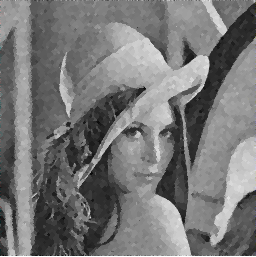
\includegraphics[width=0.4\textwidth]{007}}
\subfigure[TV复原算法所得结果]{\label{figure:1} 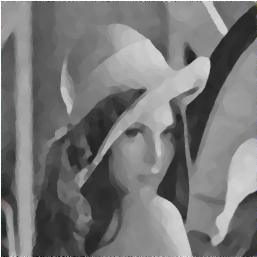
\includegraphics[width=0.4\textwidth]{008}}
\end{figure}
取 $\lambda=\frac{10}{20^2},\epsilon=0.00001$,迭代 $50$ 次。以下是所得结果:
\begin{figure}[H]
\centering
\subfigure[本文算法所得结果]{\label{figure:1/2} 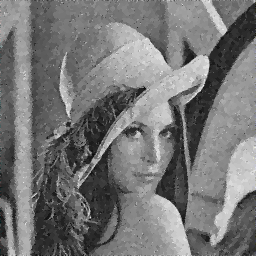
\includegraphics[width=0.4\textwidth]{009}}
\subfigure[TV复原算法所得结果]{\label{figure:1} 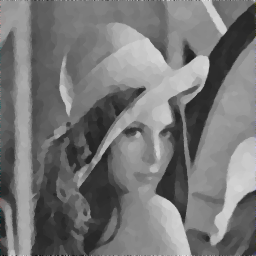
\includegraphics[width=0.4\textwidth]{010}}
\end{figure}
从上结果可以看出在相同参数条件下,本文算法相对于TV复原算法对于边缘的保持较好。



